% !TEX root = ../thesis.tex
\section{Augmentace dat}
\label{chap:realisation:augmentation}

Poslechový test jasně ukázal, že správné rozpoznání pronesené EL promluvy není lehký úkol ani pro člověka. Naprosto markantní význam hraje kontext. Ten pomáhá, pokud některá část promluvy nebyla dobře rozumnět nebo bylo těžké ji porozumnět. Navíc, ze zkušeností získaných při pořizování řečového korpusu (části \ref{chap:construction:corpus} a \ref{chap:realisation:corpus}), plyne, že EL řečník má tendenci mluvit ve spíše kratších dávkách slov, mezi kterými dělá drobné pauzy. Pro člověka není problém udržet v povědomí kontext, ale stroji to může někdy způsobovat problémy. Otázkou tedy je, jak \uv{vylepšit} stroj tak, aby poskytoval lepší výsledky?

Ať se řečník snaží sebevíc, tak se současnými metodami rehabilitace hlasu (viz \ref{chap:cause:treatment}), se při ztrátě hlasivek část informace z produkované řeči ztrácí. V poslední době bylo prezentováno několik přístupů jak ztracenou informaci obnovit. Souhrn těch nejperspektivnějších je v \cite{Denby2010}. Ve valné většině případů se využívá obohacení akustického modelu o artikulační data, nebo dokonce využití jen těchto artikulačních dat. \cite{Hofe2013} Problém ale spočívá v tom, že ne všechny akustické nuance mezi podobnými fonémy jsou artikulací ovlivněny. Navíc její záznam s sebou často nese používaní dalšího zařízení (kamery, ultrazvuku, atp. \cite{Hueber2010}), nebo dokonce nutnost podstoupení dalšího operačního zákroku (magnety \cite{Hofe2011}). Samozřejmě je férové říct, že většina těchto vyvíjených systémů si klade za cíl komletně nahradit současné metody rehabilitace. Na druhou stranu faktem je, že ani po dlouholetém vývoji se většina těchto systémů nedostala z raně vývojové fáze. Nepochybně hraje roli, že je tato problematika přeci jen na okraji zájmu řečařské komunity.

Pokud tedy není úplně reálné získat ztracenou informaci pomocí kompletní změny paradigmatu fungování systémů rozpoznávání řeči, tak zbývá jen pracovat s informací, která je k dispozici a adaptovat současný model. Určitou možností je nahrazení ztracené informacé konkrétní cílenou změnou produkované řeči. Řečník by ideálně neměl být touto změnou ovlivněn. Jako optimální se jeví změna produkované řeči, která je zohledněna modelem. Samozřejmě takovýto přístup nezbavý řečníka EL, ale může mu pomoci v situacích, které jsou pro něj stresující a v konečném důsledku mu velmi komplikují život.

Jako nejjednodušší možnost augmentace se jeví protežení určitých fonémů. Člověk je naprosto bez problémů schopen měnit tempo promluvy. Dokonce velmi často se děje mimoděk, protože tempo řeči velmi významně závisí na emočním a fyzickém stavu jedince. Pokud by se řečník naučil automaticky protahovat určité fonémy, teoreticky by to mohlo pomoci při rozpoznávání. U HMM modelů se délka fonému modeluje pomocí přechodu ze stavu $s_x$ do stejného stavu $s_x$, viz \ref{chap:asr:acoustic:HMM}. Z výsledků \uv{bigrams} experimentu (část \ref{chap:realisation:listening:bigrams}) se dá usuzovat, že modely fonémových párů lišících se znělostí jsou si velmi podobné. Protažení jednoho fonému z inkriminovaného páru může vést k lepšímu odlišení těchto modelů
%situaci, že modely si nebudou tolik podobné, protože se změní pravděpodonost přechodu ze stavu $s_x$ opět do stavu $s_x$.
a tím pádem vyšší přesnosti rozpoznání.
%Teorie je jedna věc, ale praxe je věc druhá.

K ověření jsou potřeba data. Bohužel získání reálných dat je zdlouhavý proces (viz \ref{chap:construction:corpus} a \ref{chap:realisation:corpus}), navíc není zřejmé jestli se vůbec vyplatí je pořizovat, protože se jedná o hypotézu. Mnohem prozaičtěji se jeví možnost uměle data protáhnout v místech výskytu zajmových fonémů. Toto protažení je teoreticky možné realizovat dvěma způsoby:

\begin{enumerate}
  \item protažení na příznacích
  \item protažení na zvuku
\end{enumerate}

\noindent V obou případech je nezbytné získat co možná nejpřesnější fonetické zarovnání. Pokud bude obsahovat chyby, tak mohou být protahovány úplně jiné úseky řeči. K natrénování HMM-DNN modelu je zapotřebí zarovnání získané HMM-GMM modelem, viz \ref{chap:asr:acoustic:DNN}. Zarovnání je však možné získat i z HMM-DNN modelu. Je tedy vhodné použít model s nejvyšší dosaženou přesností. U obou variant protažení je postup stejný:

\begin{enumerate}
  \item natrénování akustického modelu na originálních datech.
  \item získání zarovnání.
  \item protažení zájmových fonémů podle zarovnání.
  \item natrénování nového akustického modelu na protažených datech.
\end{enumerate}

\noindent Nový model může být otestován a výsledky porovnány s těmi dosavadními. Tyto modely navíc pomohou určit vhodné parametry pro případné skutečné protažení dat.

%V následujícím textu je nejprve v části \ref{chap:realisation:augmentation:features} popsáno jakým způsobem je realizováno protažení na příznacích a následně je vytvořena sada modelů, která je otestována. V části \ref{chap:realisation:augmentation:audio} je stejným způsobem popsáno protažení na audio nahrávkách, ze kterých jsou natrénovány a otestovány modely.

\subsection{Protažení na příznacích}
\label{chap:realisation:augmentation:features}

Protažení na příznacích vychází z představy, že při protažení (např. fonému) a následné parametrizaci, budou v inkriminovaných mikrosegmentech po sobě následovat velmi podbné příznakové vektory.
%po sobě protažen, tak po parametrizaci, oproti neprotaženémé promluve, po sobě následují velmi podobné příznakové vektory.
%Tzn. změna příznakových vektorů není tak markatní.
Teoreticky, v krajním případě, by mohlo dojít i k tomu, že část ptěchto příznakových vektorů je idenckých. Pokud je tedy cílem zjistit, zda protožení může pomoci při rozpoznávání EL řeči, tak je možné (teoreticky) docílit protažení zkopírováním určitých příznakových vektorů
%a tím docílit \uv{protažení}.
Lépe je tato myšlenka ilustrována obr. \ref{fig:realisation:augmentation:features}. Nejprve je nahrávka standardně zparametrizována. Barevně jsou vyznačeny případné vektory odpovídající zájmovému úseku (tedy fonému). Konrétní hranice jsou získány ze zarovnání. Tyto vektory jsou pak zduplikovány a tím je \uv{dosaženo} dvojnásobného protažení.

\begin{figure}[hbpt]
  \centering
  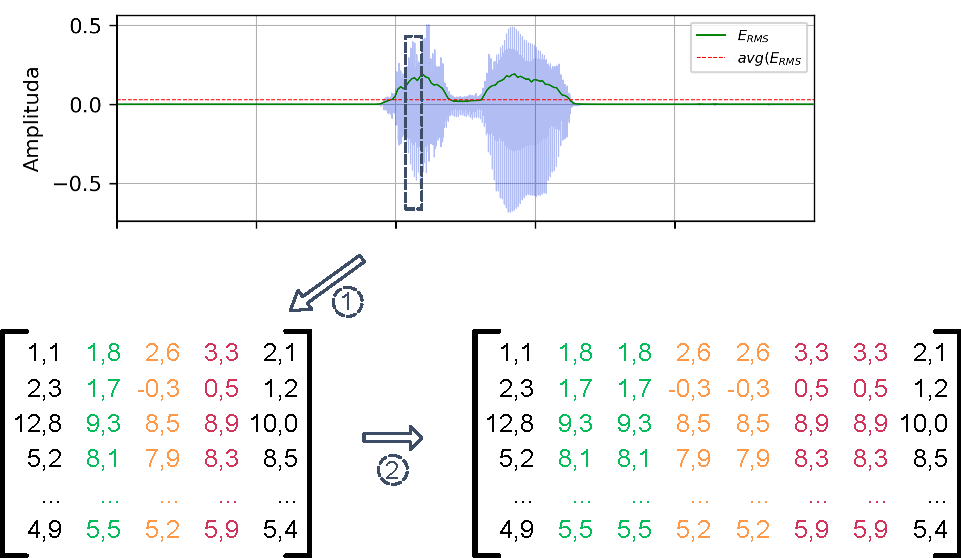
\includegraphics[width=0.9\textwidth]{./ch5-construction/img/augmentation_features.pdf}
  \caption{Princip protažení na příznacích.}
  \label{fig:realisation:augmentation:features}
\end{figure}

Toto protažení je však spíše hypotetická možnost. V reálné situaci by řečník mluvil jako doposud a k protažení by docházelo při zpracování. Což je velmi netriviální úkol. Teoreticky by se musel algoritmus parametrizace doplnit o mechanismus, který by určité příznakové vektory určitým způsobem duplikoval. Prosté zkopírování navíc porušuje dynamický charakter řeči. V rámci jednoho zpracovávaného mikrosegmentu jsou parametry považovány za statické, ale jak se okénko v rámci zpracování posouvá, tak už nelze hovořit o stacionaritě parametrů. Tento problém by se musel řešit nějakým druhem interpolace mezi dvěma konsekutivními vektory. Mechanismus by zároveň vyřešil omezení, kdy je kopírováním možné získat pouze protažení odpovídající celočíselnému násobku původní délky. Proč tedy vůbec zkoušet tento typ protažení? Odpověď je jednoduchá, nehraje zde takovou roli přesnost zarovnání. V průběhu zpracování je využíváno posuvného okénka a překryvu. Díky tomu dojde k určitému \uv{rozmazání} hranic. Pro prvotní experimenty je to pak relativně vhodné zjednodušení úlohy.

\subsubsection{Dosažené výsledky}

Prvním bodem výše zmíněného algoritmu je získání standardního modelu, který je použit k zarovnání dat. K tomu je možné použít již natrénovaný model z experimentů popsaných v části \ref{chap:realisation:corpus:elimination}. Konrétně se jedná o HMM-DNN model s $5$ skrytými vrstvami, každá s $4096$ neurony. Výstupní vrstva je pak typu softmax dimenze rovné počtu HMM stavů. Tento model dosáhl s fonémovým zerogramovým LM přesnoti $84,66\ \%$. S jeho pomocí je získáno zarovnání trénovací i testovací sady.

Jako prvotní ověřovací experiment je zvoleno dvojnásoné protažení fonému $/s/$. Jinými slovy, všechny vektory odpovídající $/s/$ jsou zduplikovány. Následně je standardním způsobem natrénován HMM-DNN model. Neuronová síť má $5$ skrytých vrstev s $4096$. Výstupní vrstva je typu softmax. Otestování je jako v předchozích případech realizováno na testovací sadě s fonémovým zerogramovým jazykovým modelem, aby byl minimalizován vliv LM. Tento nový model dosáhl přesnosti $85,11\ \%$, což je malé zlepšení oproti baseline HMM-DNN modelu.

Protažení $/s/$ posloužilo k ověření procesu vytváření modelu. Další experiment je realizován na protažených fonémech $/k/$, $/p/$, $/s/$, $/t/$ a $/v/$, což představuje většinu neznělých zájmových fonémů. Zarovnání je identické jako u předchozího experimentu. Opět je uvažováno dvojnásobné protažení. Všechny vektory inkriminovaných fonémů jsou zduplikovány. Znovu je natrénován HMM-DNN model se stejnámi parametry. Model je otestován s fonémovým zerogramovým jazykovým modelem. Přesnost na testovací sadě dosáhla hodnoty $87,50\ \%$, což lze považovat za významné zlepšení.

Doposud se uvažovalo pouze dvojnásobné protažení, v další fázi je tedy potřeba oveřit jestli jiné hodnoty nemohou poskytnout lepší výsledek. Celkem je uvožované $3x$, $4x$ a $5x$ protažení. Protaženy jsou fonémy $/k/$, $/p/$, $/s/$, $/t/$ a $/v/$. Proces natrénování a otestování modelu je stejný jako v předchozích případech. Dosažené výsledky jsou pak v tab. \ref{tab:realisation:augmentation:influence}. Pro úplnost je tabulka doplněna o baseline model s $1x$ protažením a již prezentované $2x$ protažení. Z výsledků je patrný jasný trend, větší než $2x$ protažení vede ke zhoršení přesnosti. Optimální hodnota protažení tak teoreticky leží někde v intervalu $\left(1,\ 3\right)x$. Bohužel s protahovaním pomocí kopírování příznakových vektorů není možné přesné určení hodnoty.

\begin{table}[htpb]
  \centering
  \def\arraystretch{1.5}
  \pgfplotstabletypeset[
    col sep=semicolon,
    string type,
    columns/extension/.style={
      column name={},
      column type={l},
      string replace={accp}{$Acc_{p}\ [\%]$}
    },
    columns/1x/.style={column name=1x, column type={r}},
    columns/2x/.style={column name=2x, column type={r}},
    columns/3x/.style={column name=3x, column type={r}},
    columns/4x/.style={column name=4x, column type={r}},
    columns/5x/.style={column name=5x, column type={r}},
    every head row/.style={
      after row={
        % \cmidrule{2-10}
        \midrule
      },
      before row={\toprule & \multicolumn{5}{c}{Míra protažení} \\}
    },
    every last row/.style={after row={\bottomrule}},
  ]{./ch5-construction/tabs/0301-features.csv}
  \caption{Vliv míry protažení na přesnost modelu.}
  \label{tab:realisation:augmentation:influence}
\end{table}

Zhoršení přesnosti u vyšších hodnot protažení dozajista souvísí s faktem, že výsledná augmentovaná data neodpovídají realitě. Čím vícekrat je vektor zkopírován, tím více je vnášena chyba způsobená ignorováním dynamické povahy signálu. Nicméně jako proof-of-concept myšlenky posloužil tento experiment velmi dobře.
%Protažení na příznacích vede ke zvýšení přesnosti a má smysl tuto cestu více prozkoumat.

\subsection{Protažení na zvuku}
\label{chap:realisation:augmentation:audio}

Protažení na příznacích vedlo k významnému zlepšení, ale tento přístup není bohužel reálně použitelný. Tím může být až model pracující s fonémy protaženými přímo v audiu signálu. Tato data budou teoreticky více odpovídat reálným datům získaným od řečníka.

Stejně jako v předchozím případě je k protažení potřeba zarovnání. To s určitou mírou přesnosti určuje počáteční a koncové hranice jednotlivých fonémů. Na základě je možné určitý úsek protáhnout například pomocí:

\begin{itemize}
  \item převzorkování signálu,
  \item TD-PSOLA algoritmu,
  \item fázového vokodéru.
\end{itemize}

\noindent Asi nejednodušší je převzorkování dat, stačí načíst všechny vzorky odpovídající vybranému fonému a změnit vzorkovací frekcenci. Pokud je cílem úsek protáhnout, je výsledná nová vzorkovací frekvence menší než originální. Hlavním problémem této metody je tonální posun\footnote{Mění se fundamentální frekvence $F_0$. Pokud dojde ke zrychlení, frekvence se zvýší. Při zpomalení naopak sníží.}. Cílem je protáhnout konrétní foném, který z celkové délky nahrávky zabírá jen malou část. Proto by se dal tento nepříznivý jev ignorovat. Snaha je však vygenerovat co možná nejreálnější protažené nahrávky, a proto není protažení pomocí převzorkování nejvhodnější metodou.

Zbylé dva uvažované přístupy umožňují sofistikovanější úpravy signálu. Snahou je upravit časové vlastnosti signálu aniž by byl nepříznivě ovlivněn tón.  Obě metody využívají \textit{analýzy} signálu,  následováné \textit{zpracováním} a zakončené \textit{syntézou}. Rozdíl je hlavně ve způsobu. Metody z rodiny \textit{PSOLA} pracují s hlasivkovými pulsy, které jsou nejprve v analytické části nalezeny\footnote{Výsledkem analýzy jsou periodicky se opakující značky, angl. pitch marks. Úpravou jejich parametrů dochází ke změnám parametrů řeči.}, aby pak v části zpracování došlo k jejich transformaci na základě požadavků na výslednou řeč. V posledním kroku dochází k syntéze signálu na základě upravených analytických krátkodobých signálů, tedy hlasivkových pulsů. Více detailnějí se o této metodě hovoří v \cite{Psutka2006}.

Fázový vokodér pracuje na podobném principu, s tím rozdílem, že v analytické části dochází k převodu signálu do frekveční oblasti pomocí FFT. Ve fázi zpracování je signál upraven, aby ve fázi syntézy byl opět převeden do časové oblasti pomocí inverzní FFT.

Pomocí těchto dvou zmíněných metod je možné upravit nejen délku, ale i $F_0$ signálu. Stejně jako u převzorkování mají neblahý vliv na signál, ale ten není tak markantní jako v případě převzorkování. U \textit{TD-PSOLA} mohou například vznikat artefakty způsobnené nespojitostmi mezi sousedními upravenými úseky řeči. U fázového vokodér nevznikají artefakty vlivem nespojitostí, ale vlivem fázového posunu.

%Jelikož se signál upravuje ve frekveční oblasti, kde dochází ke změnám jednotlivých komponent, může dojít k fázovému posunu mezi jednotlivými komponentami. Při syntéze pak mohou vznikat zaznamenatelné artefakty připomínající tupý zvuk.

Obě metody však poskytují velmi dobré výsledky protažená na jednotlivých fonémech. Výsledné protažení je téměř identické. Interně vyvinutý nástroj umožňující ovlivnění délky řeči (a priory používaný při syntéze řeči) poskytuje obě zmíněné metody. Pro výsledné protažení je použita metoda \textit{TD-PSOLA}. Ukázka původního a protaženého slova \uv{kosa} je na obr. \ref{fig:realisation:augmentation:compare}. Protahován byl foném $/s/$, který je v signálu vidět jako šum mezi dvěmi výraznými častmi signálu. Inkriminovaný foném byl protažen na dvojnásobek. Na obr. \ref{fig:realisation:augmentation:compare:augmented} je pak zřetelně vidět protažení úseku odpovídající $/s/$. V signálu a ve spektru není vidět žádný významný artefakt.

\begin{figure}[htpb]
  \centering
  \begin{subfigure}[b]{0.42\textwidth}
    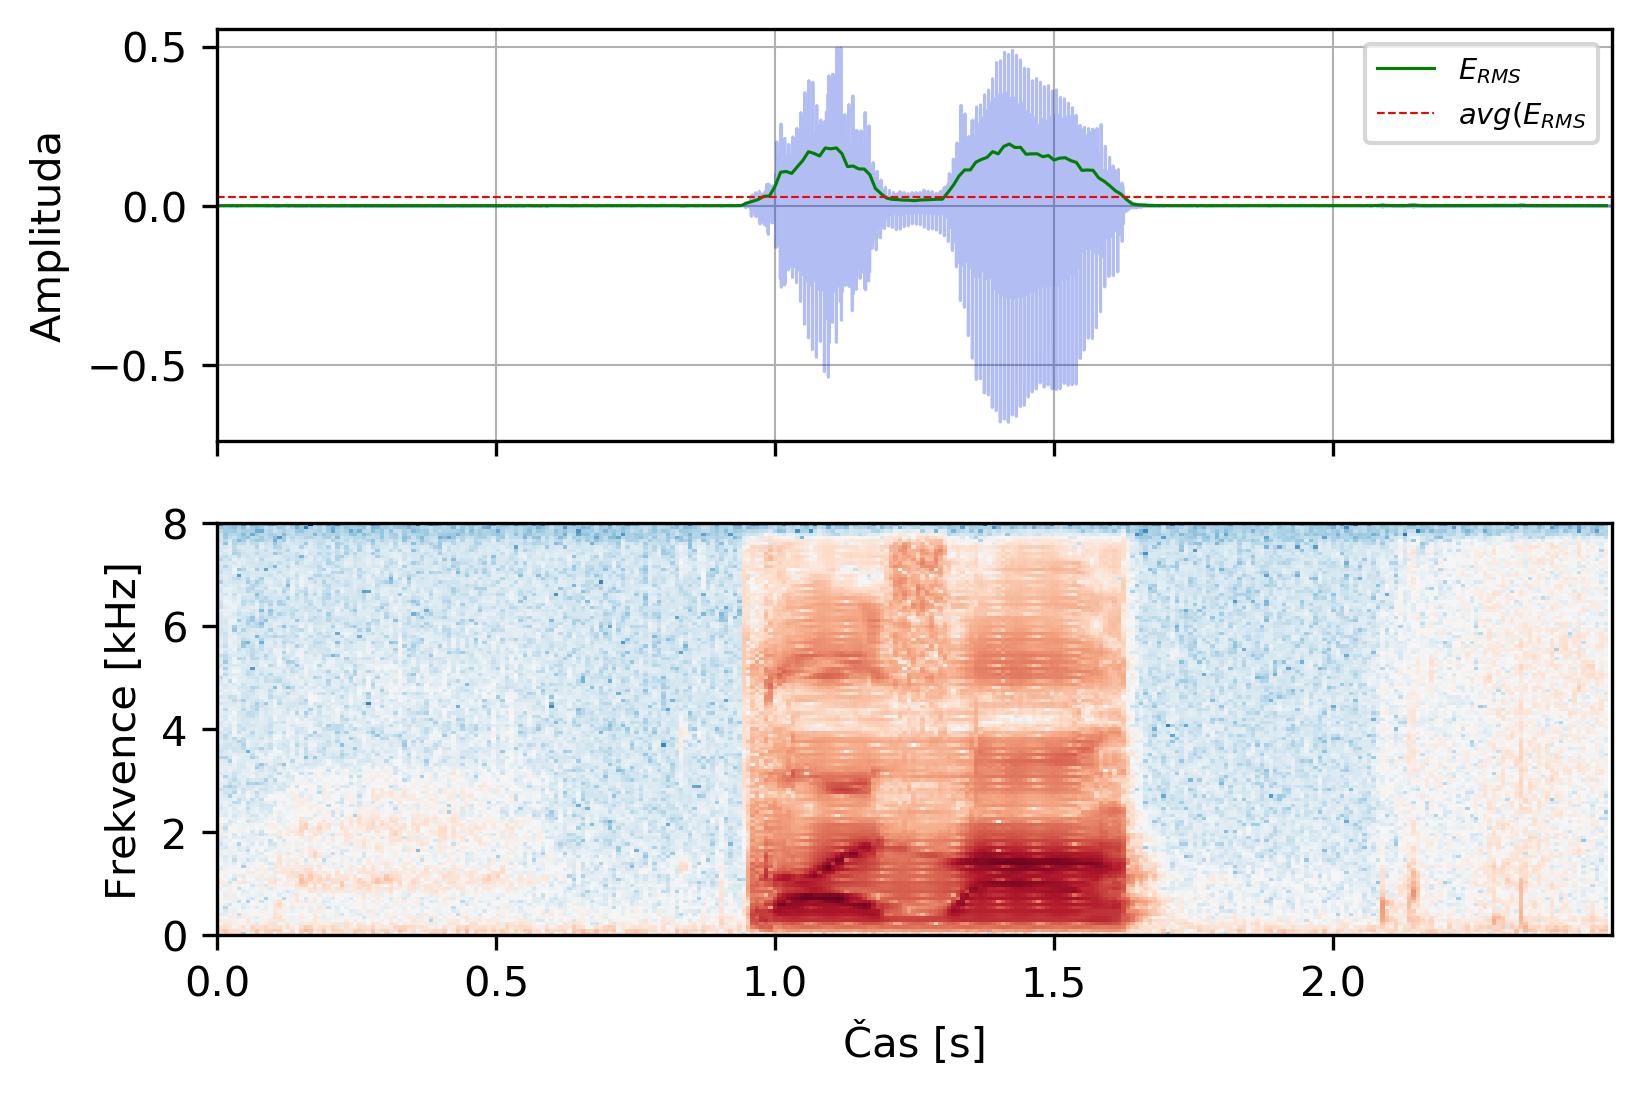
\includegraphics[width=\textwidth]{./ch5-construction/img/energy_spec_word-normal.png}
    \caption{Originální}
    \label{fig:realisation:augmentation:compare:original}
  \end{subfigure}
  %
  \begin{subfigure}[b]{0.42\textwidth}
    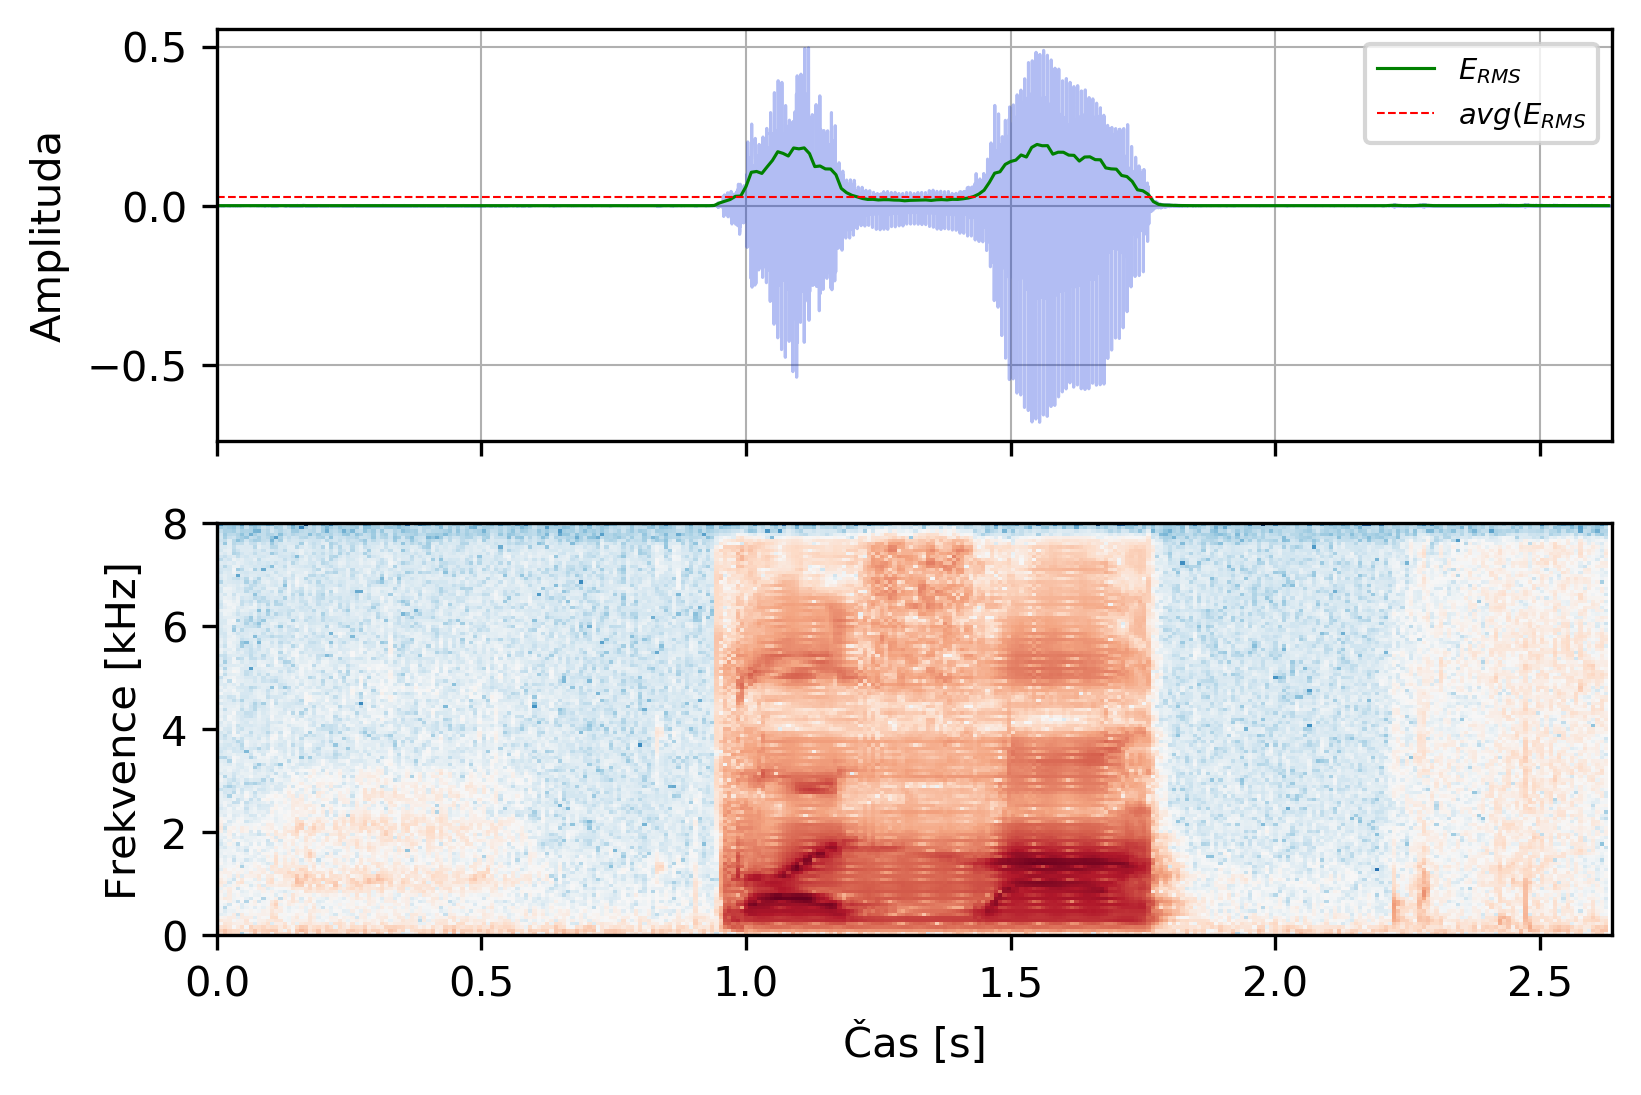
\includegraphics[width=\textwidth]{./ch5-construction/img/energy_spec_word-augmented.png}
    \caption{Protažené}
    \label{fig:realisation:augmentation:compare:augmented}
  \end{subfigure}
  \caption{Amplituda a spektrogram původního (protaženého) slova \uv{kosa}.}
  \label{fig:realisation:augmentation:compare}
\end{figure}

\subsubsection{Dosažené výsledky s DNN}

K ověření schopností modelu pracovat s uměle protaženými daty je použit stejný HMM-DNN model jako v předchozích případech. Neuronová síť má $5$ skrytých vrstev, každá s $4096$ neurony. Výstupní vrstva je pak typu softmax dimenze rovné počtu HMM stavů. Vstupní data jsou zparametrizována pomocí PLP (12 statických kepstrálních koeficientů společně s delta a delta-delta parametry). V datech jsou protaženy všechny výskyty fonémů $/k/$, $/p/$, $/s/$, $/t/$ a $/v/$. Uvažováno je protažení $1,25x$, $1,50x$, $1,75x$ a $2,00x$. Jazykový model je stejně jako v případě protažení na příznacích fonémový zerogramový. Dosažené výsledky jsou vypsány v tab. \ref{tab:realisation:augmentation:influence:dnn}. Nejlepšího výsledku dosáhl \textit{baseline} model s hodnotou $84,66\ \%$. S libovolným protažením dochází k poklesu přesnosti.

\begin{table}[htpb]
  \centering
  \def\arraystretch{1.5}
  \pgfplotstabletypeset[
    col sep=semicolon,
    string type,
    columns/extension/.style={
      column name={},
      column type={l},
      string replace={accp}{$Acc_{p}\ [\%]$}
    },
    columns/100/.style={column name={1,00x}, column type={r}},
    columns/125/.style={column name={1,25x}, column type={r}},
    columns/150/.style={column name={1,50x}, column type={r}},
    columns/175/.style={column name={1,75x}, column type={r}},
    columns/200/.style={column name={2,00x}, column type={r}},
    every head row/.style={
      after row={
        % \cmidrule{2-6}
        \midrule
      },
      before row={\toprule & \multicolumn{5}{c}{Míra protažení} \\}
    },
    every last row/.style={after row={\bottomrule}},
  ]{./ch5-construction/tabs/0302-audio_1.csv}
  \caption{Vliv míry protažení fonému na přesnost \textit{DNN} modelu.}
  \label{tab:realisation:augmentation:influence:dnn}
\end{table}

\subsubsection{Upravené zarovnání a time delay neural network}

Při analýze výsledků se ukázalo, že zarovnání v mnoha případech není zrovna nejpřesnější a to zvláště u inkriminovaných neznělých fonémů. Na obr. \ref{fig:realisation:augmentation:alignemnt:wrong} je získané zarovnání slova \uv{kosa} společně s vyznačenými hranicemi v audiu signálu a spektru. Z obr. \ref{fig:realisation:augmentation:alignemnt:wrong:audio} je zřejmé, že počáteční hranice $/s/$ zasahuje do předchozího fonému $/o/$. Tím pádem dochází k protažení nevhodné části signálu a model se tak učí na špatných datech. Pokud by všechny fonémy $/s/$ následovaly po $/o/$, tak by se nejednalo o závažný problém, ale toto samozřejmě neplatí.

\begin{figure}[htpb]
  \centering
  \begin{subfigure}[b]{0.26\textwidth}
    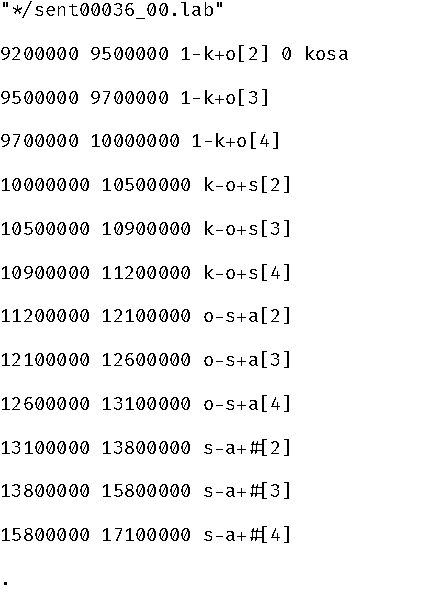
\includegraphics[width=\textwidth]{./ch5-construction/img/alignment_text.pdf}
    \caption{Zarovnání}
    \label{fig:realisation:augmentation:alignemnt:wrong:text}
  \end{subfigure}
  %
  \begin{subfigure}[b]{0.55\textwidth}
    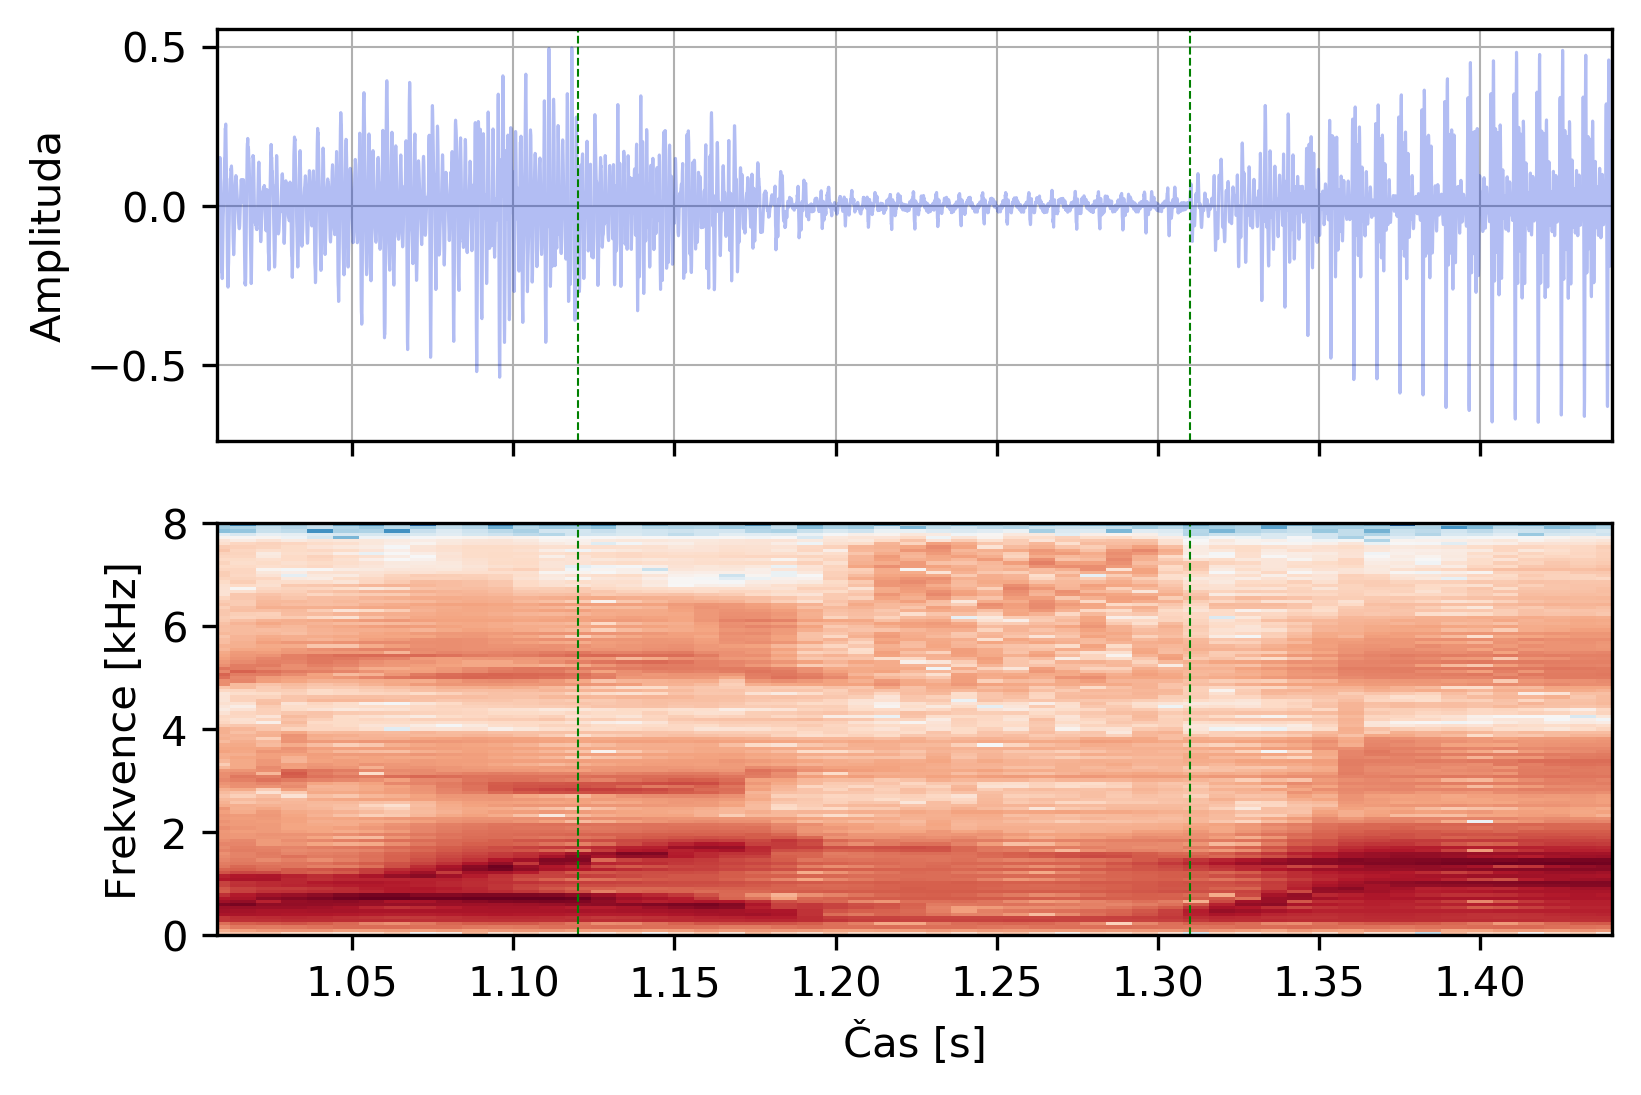
\includegraphics[width=\textwidth]{./ch5-construction/img/energy_spec_word-segment.png}
    \caption{V signálu}
    \label{fig:realisation:augmentation:alignemnt:wrong:audio}
  \end{subfigure}
  \caption{Špatně zarovnaný foném $/s/$ ve slově \uv{kosa}.}
  \label{fig:realisation:augmentation:alignemnt:wrong}
\end{figure}

%Pro lepší zarovnání je potřeba upravit model, který se o zarovnání stará. \todo{TBD}{Doplnit vysvětlení od Pepika.}

V době experimentů s protažením konkrétních fonémů se začaly stále více prosazovat time-delay neural networks (\textit{TDNN}) . Přestože patří do rodiny feed-forward sítí jako DNN, tak oproti nim se snaží vzít v potaz i dynamickou složku řeči, více o rozdílu mezi DNN a TDNN v části \ref{chap:asr:acoustic:DNN}.
%U \textit{DNN} jsou všechny neurony v jednotlivých vrstvách propojeny a tedy vstupní vektor je zpracováván všemi neurony v následující vrstvě. U \textit{TDNN} toto neplatí, neurony v určité vrtvě jsou propojeny vždy jen s určitým počtem neuronů ve vrstvě následující, viz obr. \ref{fig:experiments:augmentation:tdnn}. To v důsledku znamená, že části sítě vykonávájí rozhodnutí na základě jiných podmnožin vstupních dat. V dalších vrstvách se pak tyto lokální rozhodnotí integrují, aby na výstupu sítě došlo ke globálnímu rozhodnutí. Tedy, aby byl výstupem sítě foném odpovídající času $t_c$ a jeho okolí $\langle t_{c-n}; t_{c+m} \rangle$.

% S posunem okénka velikosti $m + n + 1$ postupně jednotlivé části sítě zpracují všechny části vstupního zparametrizovaného signálu. Dynamika je zohledněna další množinou vah, která se mění podle toho jakou část vstupního vektoru ta část sítě zpracovává \cite{Waibel1989}. Tento přístup by se dal přirovnat ke konvoluční neuronové síti (\textit{CNN}), kde se také vstupní data (většinou obrázky) nezpracovájí najednou, ale pomocí filtrů vždy jen malá podmnožina. A v dalších vrstvách dochází ke spojování výsledků z těchto podmnožin. Hlavní rozdíl mezi \textit{TDNN} a \textit{CMN}  je v tom, že \textit{CMN}  nepracuje s konceptem času. Více množin vah lze považovat za určitý ekvivalent paměti u RNN sítí.

% \begin{figure}[hbpt]
%   \centering
%   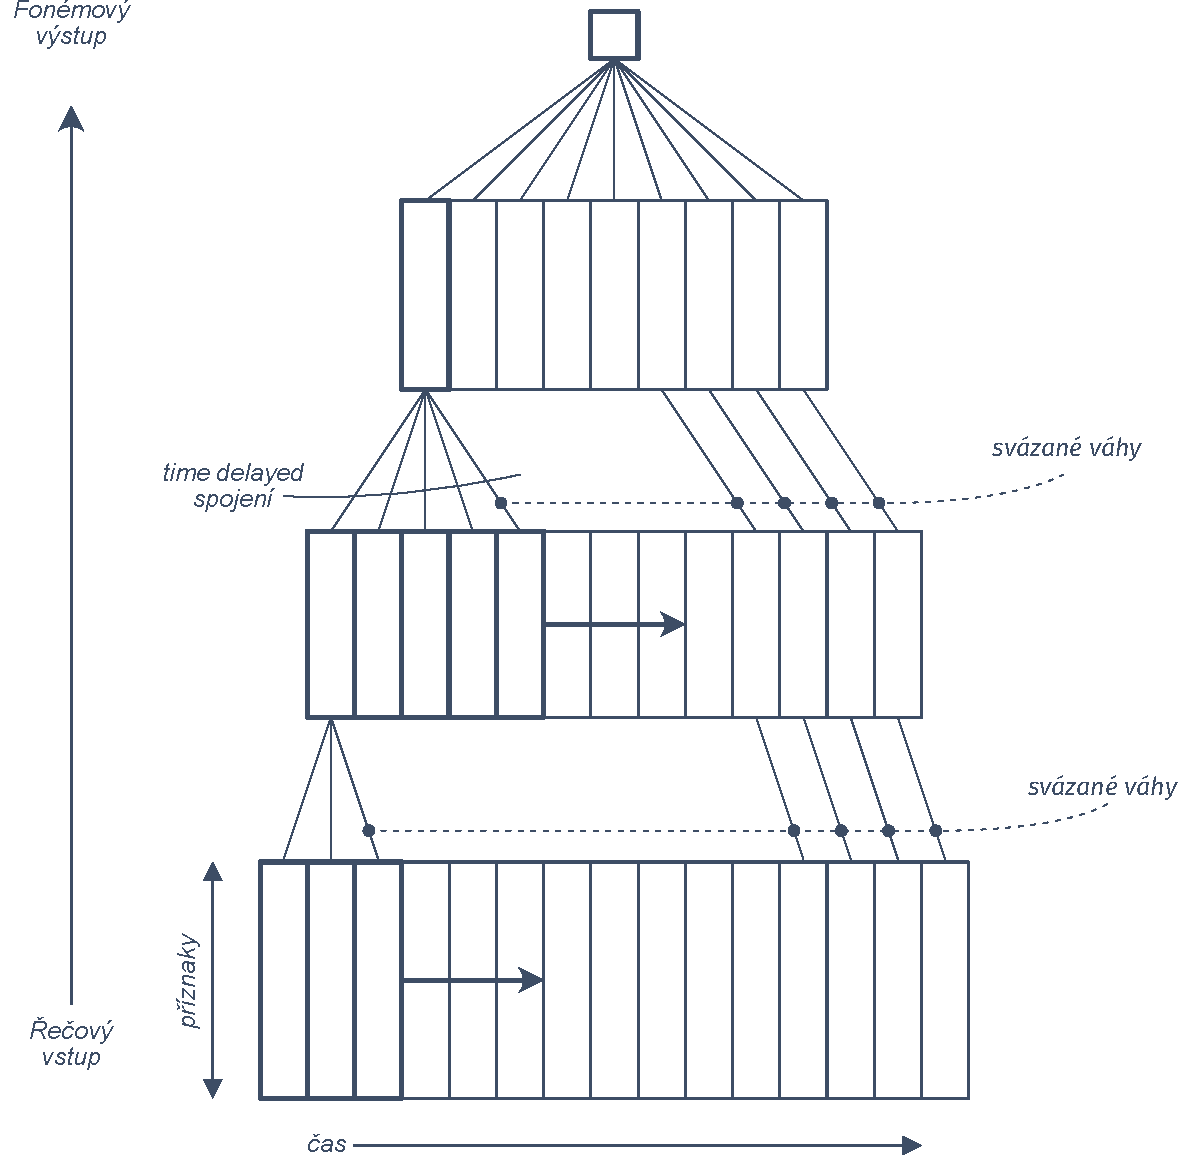
\includegraphics[width=0.5\textwidth]{./ch5-construction/img/tdnn.pdf}
%   \caption{Time delay neural network (\textit{TDNN}) .}
%   \label{fig:experiments:augmentation:tdnn}
% \end{figure}

Stejně jako u DNN moelu je na počátku trénování nutné mít k dispozici zarovnání. To, ale nemusí být naprosto přesné, protože je vstupní vektor zpracováván jiným způsobem než u DNN. Díky FIR filtraci a více množin vah je brán v potaz i dynamický charakter řeči \cite{Peddinti2015}. Model založený na TDNN by tak měl generovat přesnější zarovnání a tím zlepšit výsledky modelu pracující s uměle protaženými daty.

Jako startovní bod trénování je použito DNN zarovnání z předchozího experimentu. Topologie sítě vychází z hodnot prezentovaných v \cite{Peddinti2015}, tedy síť má $4$ skryté vrstvy. Každá vrstva má 650 neuronů. První vrstav pracuje s kontextem $t-2$ a $t+2$, druhá vrstva s $t-1$ a $t+2$, třetí vrstva s $t-3$ a $t+4$ a čtvrtá s $t-7$ a $t+2$. Výpočet výstupu pak bere v potaz kontext $t-13$ a $t+9$ mikrosegmentů, viz \cite{Peddinti2015}.

%Ukázka zarovnání získané touto sítí je zobrazena na obr. \ref{fig:realisation:augmentation:alignemnt:correct}.

Na obr. \ref{fig:realisation:augmentation:alignemnt:correct} je zonrazeno získané zarovnání slova \uv{kosa} TDNN modelem. Z vyznačených hranic fonému $/s/$ (obr. \ref{fig:realisation:augmentation:alignemnt:correct:audio}) je patrné v podstatě přesné zarovnání. Přesnost TDNN modelu s fonémovým zerogramovým jazykovým modelem dosáhla hodnoty $Acc_{p}= 85,41\ \%$.
%To předznamenává i lepší vlastnosti \textit{TDNN} modelu. Pro ověření této hypotézy opět poslouží standardní experiment s monofonovým zerogramovým LM.
%Z tohoto zarovnVýsledná přesnost má hodnotu $85,41\ \%$. Síť tedy dosáhla nepatrně lepšího výsledku než \textit{DNN} síť.

\begin{figure}[htpb]
  \centering
  \begin{subfigure}[b]{0.26\textwidth}
    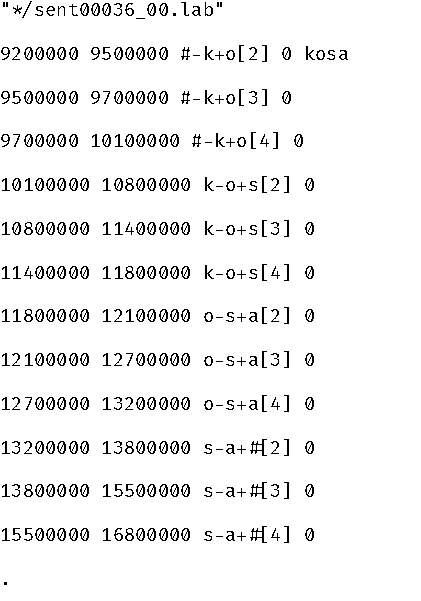
\includegraphics[width=\textwidth]{./ch5-construction/img/alignment_text-2.pdf}
    \caption{Zarovnání}
    \label{fig:realisation:augmentation:alignemnt:correct:text}
  \end{subfigure}
  %
  \begin{subfigure}[b]{0.55\textwidth}
    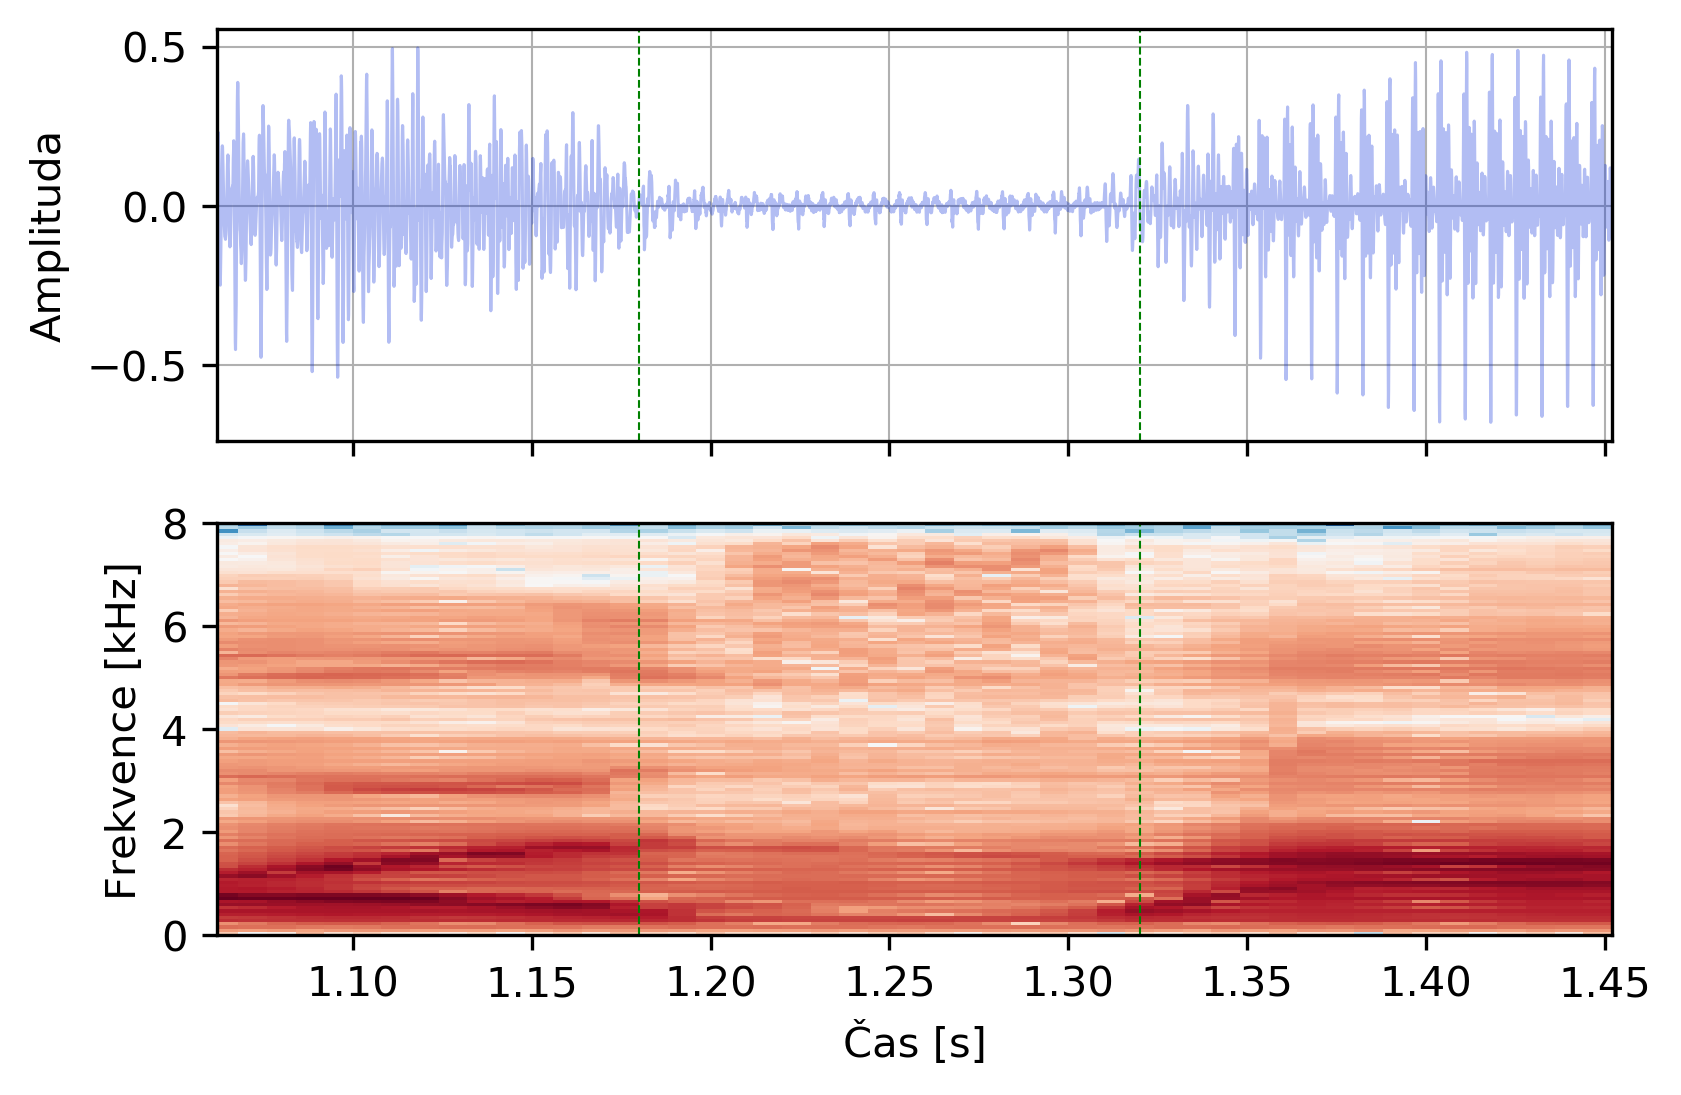
\includegraphics[width=\textwidth]{./ch5-construction/img/energy_spec_word-segment-2.png}
    \caption{V signálu}
    \label{fig:realisation:augmentation:alignemnt:correct:audio}
  \end{subfigure}
  \caption{Správně zarovnaný foném $/s/$ ve slově \uv{kosa}.}
  \label{fig:realisation:augmentation:alignemnt:correct}
\end{figure}

S relativně přesným zarovnáním je možné přistoupit k protažení fonémů $/k/$, $/p/$, $/s/$, $/t/$, $/v/$ a vytvoření nového modelu pracujícího s těmito daty. Nejprve je natrénovat HMM-GMM model, který poskytne prvotní zarovnání. V předchozích experimentech následovalo trénování DNN modelu, ale TDNN zarovnání ukázalo lepší vlastnosti tohoto modelu. Jako další model je tedy použita TDNN síť. K otestování modelu je využit standarní fonémový zerogramový jazykový model. Uvažováno je protažení od $1,25x$ do $3,00x$ s krokem $0,25$. Výsledky experimentu jsou vypsány v tab. \ref{tab:realisation:augmentation:influence:tdnn}. Oproti těm v tab. \ref{tab:realisation:augmentation:influence:dnn} je vidět výrazné zlepšení přesnoti  oproti baselinu modelu ($Acc_{p} = 85,41\ \%$. Nejvyšší přesnosti $87,90\ \%$ dosáhl model pracující s $2,5x$ protaženými daty. Navíc modely pracující s protažením od $1,75x$ do $2,75x$ dosahují velmi podobných výsledků. To poskytuje relativně široký pracovní interval pro případné skutečně protažená data řečníkem.

\begin{table}[htpb]
  \centering
  \def\arraystretch{1.5}
  \pgfplotstabletypeset[
    col sep=semicolon,
    string type,
    columns/extension/.style={
      column name={},
      column type={l},
      string replace={accp}{$Acc_{p}\ [\%]$}
    },
    columns/100/.style={column name={1,00x}, column type={r}},
    columns/150/.style={column name={1,50x}, column type={r}},
    columns/125/.style={column name={1,25x}, column type={r}},
    columns/175/.style={column name={1,75x}, column type={r}},
    columns/200/.style={column name={2,00x}, column type={r}},
    columns/225/.style={column name={2,25x}, column type={r}},
    columns/250/.style={column name={2,50x}, column type={r}},
    columns/275/.style={column name={2,75x}, column type={r}},
    columns/300/.style={column name={3,00x}, column type={r}},
    every head row/.style={
      after row={
        % \cmidrule{2-10}
        \midrule
      },
      before row={\toprule & \multicolumn{9}{c}{Míra protažení} \\}
    },
    every last row/.style={after row={\bottomrule}},
  ]{./ch5-construction/tabs/0303-audio_2.csv}
  \caption{Vliv míry protažení fonému na přesnost TDNN modelu.}
  \label{tab:realisation:augmentation:influence:tdnn}
\end{table}

Experimenty s uměle protaženými daty potvrdily správnost uvažované hypotézy. Protažením jednoho z párových fonému dojde k dostatečnému odlišení velmi podobných zvukových reprezentací. Tím dojde k natrénování odlišných modelů fonémů v HMM. Model pracující s fonémy protaženými přímo ve zvuku nakonec dosáhl lepších výsledků než model s uměle protaženými daty na příznacích. Svůj díl na tom má i použití TDNN modelu. Model pracující s duplikovanými příznaky naznačoval, že optimální hodnota protažení bude v intervalu $\left(1,\ 3\right)x$, což druhý typ modelu potvrdil.

\subsection{Aktualizace výsledků porovnání}
\label{chap:realisation:augmentation:comparison}

V části \ref{chap:realisation:listening} je prezentováno srovnání schopnistí člověka a stroje. Posloužily k tomu dva poslechové testy a celkem $3$ ASR experimenty \uv{onemil}, \uv{reduced} a \uv{bigrams}. S novým modelem je možné aktualizovat hypotetické výsledky stroje. Hypotetické z toho důvodu, že použitá data jsou uměle protažena. Nicméně to nebrání provedení tohoto experimentu. Získané hodnoty mohou být brány jako jakési teroretická maxima ASR systému. Uměle upravená data budou přeci jen relativně přesně a konzistentně protažena. U reálných dat toto nelze a priory očekávat.

K aktualizaci výsledků je použit nejlepší model z části \ref{chap:realisation:augmentation:audio}, tedy ten s $2,5x$ protaženými daty. Parametry experimentů jsou totožné s těmi v části \ref{chap:realisation:listening}. V případě \uv{onemil} je použit zerogramový jazykový model s 1 milionem slov, \uv{reduced} pak pouze zerogramový LM se slovy obsaženými v poslechovém testu. Speciální LM, obsahující 4 kombinace slov, je vygenerován pro každou položku \uv{bigrams} experimentu.

Dosažené výsledky jsou v \ref{tab:realisation:augmentation:comparison}. Ve všech třech experimentech došlo k významnému zlepšení. U \uv{onemil} to je $23\ \%$ absolutně, u \uv{reduced} pak $24\ \%$. K nejmarkatnějšímu zlepšení zlepšení došlu u experimentu \uv{bigrams}, dokonce $44\ \%$. Výsledky člověka jsou stejné, protože realizace poslechového testu je zdlouhavý proces a je obtížné získat dostatečný počet respondentů. Nicméně se dá očekávat, že i člověk by dosáhl zlepšení. Pokud by měl znalost o fonémech, které jsou protaženy. V opačném případě by ke zlepšení nutně nemuselo dojít, protože kromě protažení nebyl zvuk nijak pozměněn.
%Dosažené výsledky ASR systému lze brát jako teoretická maxima systému.

Velmi zajímavé je porovnání zvýšení přesnosti TDNN modelu s fonémovým zerogramovým LM ($2,49\ \%$ absolutně mezi baseline a $2,5x$ modelem) a výsledky dosaženými prezentovanými v tab. \ref{tab:realisation:augmentation:comparison}. Oproti nim je $2,49\ \%$ absolutně relativně zanedbatelné, přesto velmi významné zlepšení. Jasně to ukazuje ideu experimentů s fonémovým zerogramovým jazykovým modelem. I drobné zlepšení u akustického modelu může vést k rapidnímu zlepšení sofistikovanějšího systému.

\begin{table}[htpb]
  \centering
  \def\arraystretch{1.5}
  \pgfplotstabletypeset[
    col sep=semicolon,
    string type,
    columns/type/.style={column name=, column type={l}},
    columns/onemil/.style={column name=onemil, column type={r}},
    columns/reduced/.style={column name=reduced, column type={r}},
    columns/bigrams/.style={column name=bigrams, column type={r}},
    every head row/.style={
      after row={
        % \cmidrule(lr){1-1}
        % \cmidrule(lr){2-4}
        \midrule
      },
      before row={\toprule & \multicolumn{3}{c}{$Acc_{p}\ [\%]$} \\}
    },
    every last row/.style={
      after row={\bottomrule},
      before row={\midrule}
    },
  ]{./ch5-construction/tabs/0304-comparison.csv}
  \caption{Aktualizované porovnání dosažených výsledků člověka a stroje.}
  \label{tab:realisation:augmentation:comparison}
\end{table}

% \todo{Přidat tabulky porovnávající výsledky původního a aktualizovaného testu.}{tabulky}

\subsection{Reálně protažená data}
\label{chap:realisation:augmentation:real}

Získané výsledky s uměle protaženými daty potvrdily hypotézu, že model pracující s těmito daty může dosahovat lepších výsledků. Dalším krokem je získání reálně protažených dat. Nahrávání je relativně zdlouhavý proces, jak ukázala 1. a 2. etapa nahrávání (části \ref{chap:construction:corpus} a \ref{chap:realisation:corpus}), proto je nezbytné dobře vybrat promluvy. Problémem je navíc samotné protažení. Pokud by bylo cílem získat protažené celé slovo, lze řečníka instruovat, aby mluvil pomaleji. To, ale cílem není. Výsledné promluvy mají mít protažené pouze určité fonémy a to přibližně na dvojnásobek. Jako nejjednodušší, a svým způsobem i elegantní, se ukázal zápis se zdvojenými písmeny, které mají být protaženým fonémem, např. \uv{kossa}. Řečník je obeznámen, že pokud slovo v promluvě obsahuje tento dvojitý zápis, měl by se pokusit toto slovo patřičným způsobem protáhnout. Tento zápis navíc řečníka podvědomě \uv{nutí} vyslovit slovo jinak než v případě normálního zápisu.

Nahrávání se zhostil stejný řečník jako v 1. a 2. etapě. Tedy žena v důchodovém věku, která používá EL v běžném životě již více než 15 let. Nahrávání se uskutečnilo v průběhu 5 měsiců od července 2018 do listopadu 2018. Texty určené k nahrávání obsahavaly většinu izolovaných slov z poslechového testu a věty které doposud neobsahuje řečový korpus složený z 1. a 2. etapy nahrávání. Řečnák byl instruován, aby slova, která obsahují zdvojená pismena (např. \uv{kossa}), adekvátně prodloužil. K nahrávání byla použita stejná nahrávací místnost a aparatura jako v případě 2. etapy nahrávání (viz \ref{chap:realisation:corpus}). Nahrávací protokol byl taktéž stejný, tzn. nahrávání byl vždy přítomen operátor, který kontroloval, zda se řečník nevědomky nedopustil chyby či přeřeknutí. Stejně jako v předchozí etapě obsahuje každá nahrávka minimálně $0,5\ s$ pauzu na začátku a konci. Tato opatření významně zkracují potřebnou dobu k získání kvalitního přepisu.
%, protože po každé nahrávácí seanci je pro finální kontrolu obsahu dostatečné pouhé poslechnutí obsahu a v případě potřeby drobně poupravit přepis.
Celkem se takto v rámci 3. etapy nahrávní podařilo získat dohromady $998$ promluv obsahující věty a slova, kterých je $267$. Celkový čas promluv v 3. etapě dosáhl $2$ hodin a $28$ minut.

Na obr. \ref{fig:realisation:real:compare} je zobrazena amplituda a spektrogram slova \uv{kose} protažené řečníkem (\ref{fig:realisation:real:compare:real}) a 2x uměle (\ref{fig:realisation:real:compare:augmented}). Hlavním viditelným rozdílem je slabší zastoupení frekvencí kolem $2\ kHz$ ve spektrogramu mezi časem $3,2\ s$ a $3,4\ s$. Ač to tak na první pohled nevypadá, tak obě protažení mají téměř identickou délku $0,258\ s$ (reálné) vs. $0,261\ s$ (umělé). Vizuální rozdíl je způsoben vyšší celkovou délkou reálně protaženého slova. Foném $/s/$ je zástupcem neznělých fonémů, zdrojem je tedy a priory šum a nikoli periodický signál produkovaný hlasivkami, tím pádem je velikost amplitudy taktéž velmi podobná. Vizuální rozdíl mezi obr. \ref{fig:realisation:real:compare:real} a \ref{fig:realisation:real:compare:augmented} je způsoben vyšší maximální hlasitostí uměle protažené nahrávky, která pochází z 2. etapy nahrávání.

\begin{figure}[htpb]
  \centering
  \begin{subfigure}[b]{0.42\textwidth}
    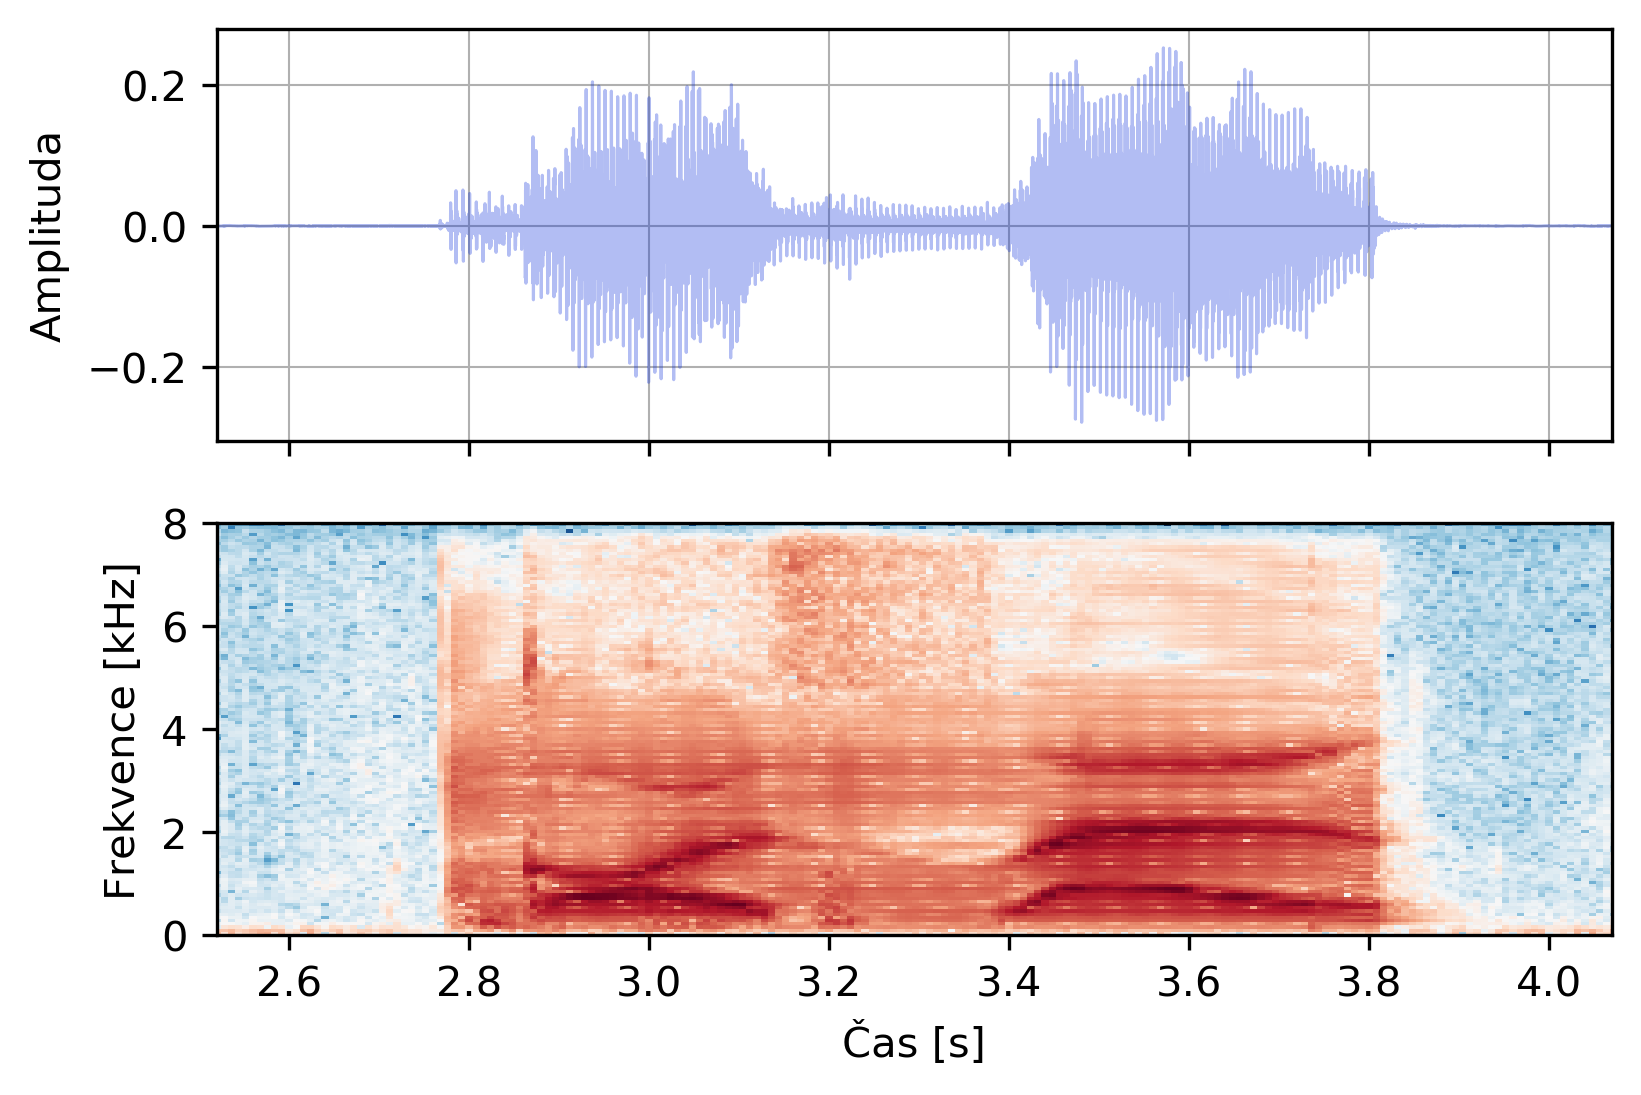
\includegraphics[width=\textwidth]{./ch6-realisation/img/energy_spec_word-kose_real.png}
    \caption{Protažené řečníkem}
    \label{fig:realisation:real:compare:real}
  \end{subfigure}
  %
  \begin{subfigure}[b]{0.42\textwidth}
    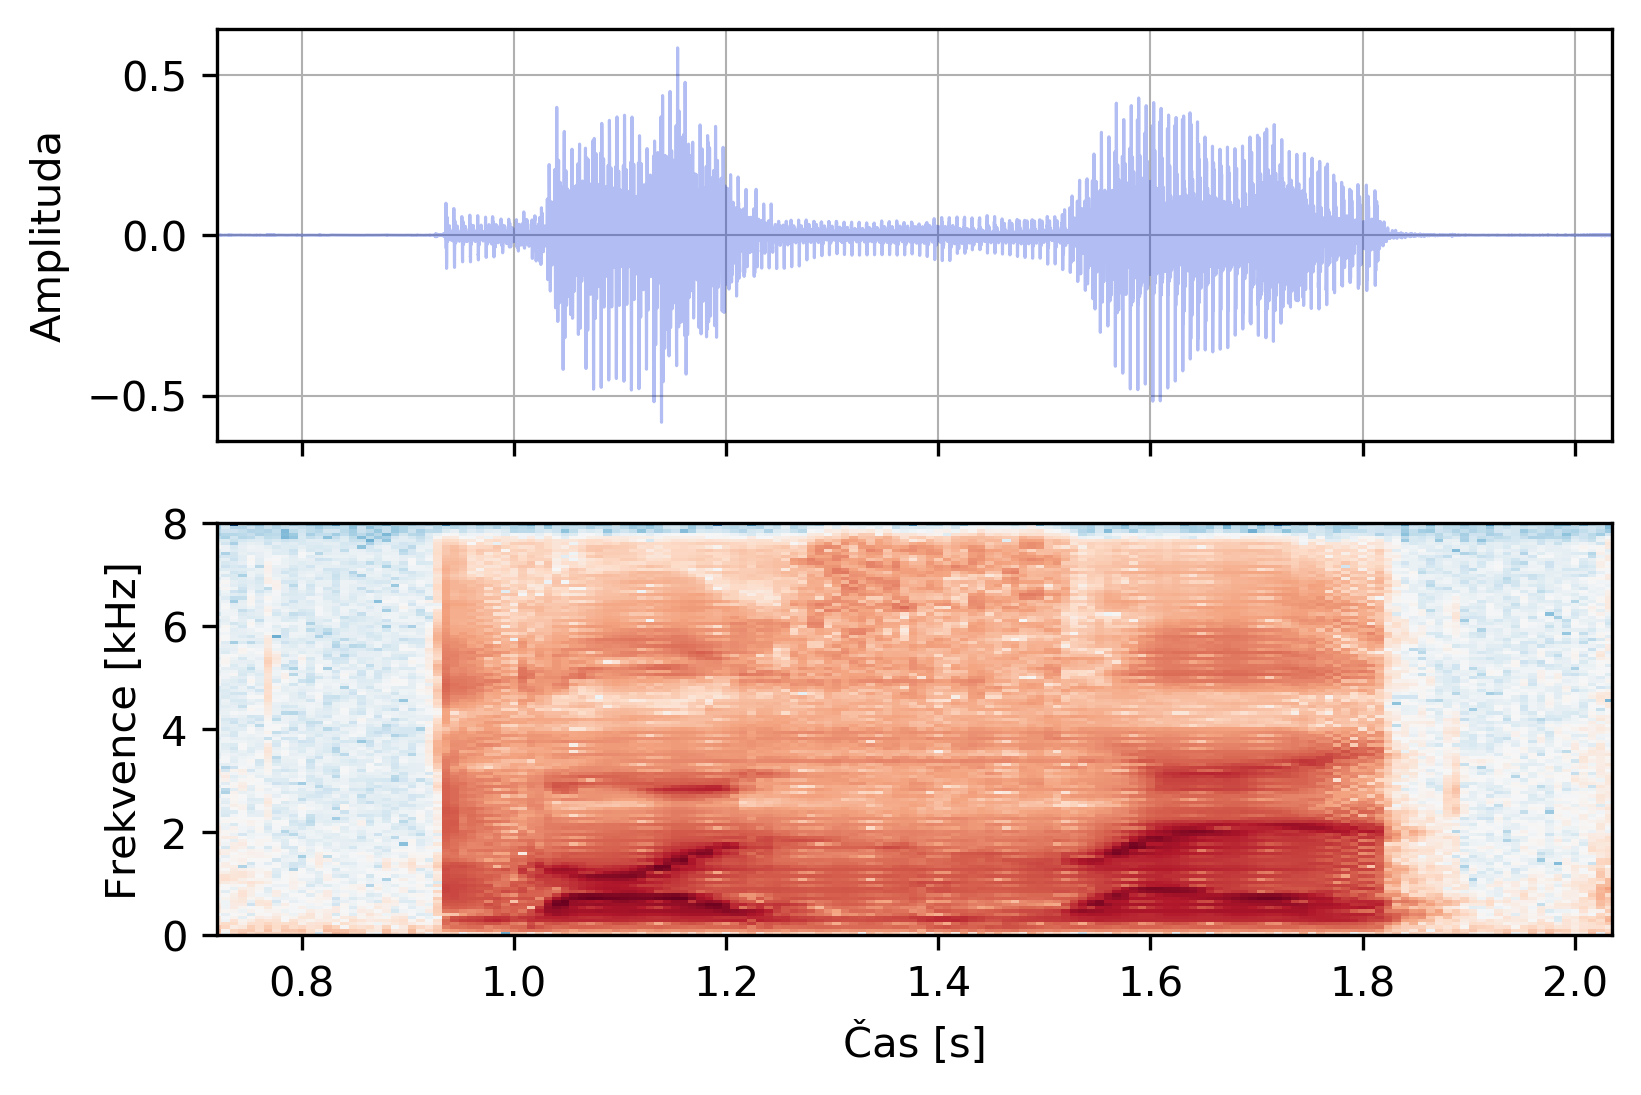
\includegraphics[width=\textwidth]{./ch6-realisation/img/energy_spec_word-kose_augmented.png}
    \caption{Uměle protažené}
    \label{fig:realisation:real:compare:augmented}
  \end{subfigure}
  \caption{Amplituda a spektrogram slova \uv{kose} protažené řečníkem/uměle.}
  \label{fig:realisation:real:compare}
\end{figure}

\begin{itemize}
  \item ukázka protažených reálných dat
  \item výsledky modelů
  \item výsledky modelu trénovaného na umělých datech, ale testovaný na reálných datech
\end{itemize}

Hlubší analýza pořízených slov ve 3. etapě nahrávání ukázala, že proces umělého protažení produkuje svými charakteristikami velmi podobné nahrávky těm reálným. Pro vytvoření modelu pouze z reálně protažených dat se však nepodařilo získat dostatečné množství dat. Pokud jsou reálně protažená data opravdu velmi podobná uměle protaženým datům, tak by mělo být možné dosáhnout \uv{dobrých} výsledků s modelem, který je natrénovaný na uměle protaažených datech, ale otestovaný těmi reálně protaženými.

Porovnáním neprotažených nahrávek z 2. etapy a protažných z 3. etapy se jako ideální jeví použití 2x protaženého modelu z části \ref{chap:realisation:augmentation:audio} (viz tab. \ref{tab:realisation:augmentation:influence:tdnn}). Jedná se tedy o TDNN model, který je natrénován z dat obsahujících 2x protažené fonémy $/k/$, $/p/$, $/s/$, $/t/$ a $/v/$.  Na testovací sadě dosáhl přesnosti $Acc_{p} = 87,71\ \%$. K otestování výkonu na reálně protažených datech jsou použity všechny věty a slova obsahující protažení zmíněných fonémů\footnote{Stejně jako u 1. a 2. etapy bylo i zde aplikováno CMN napočítané přes všechny nahrávky v rámci etapy.}. S touto testovací sadou dosáhl zmíněný model s fonémovým zerogramovým jazykovým modelem $Acc_{p} = 84,51\ \%$.

Dosažená přesnost je sice horší něž původní přesnost na uměle protažených datech, ale zároveň nedošlo k dramatickému propadu jako v případě křížového testu mezi 1. a 2. etapou (viz tab. \ref{tab:realisation:verification:cmn:full}\footnote{V tabulce jsou prezentovány hodnoty odpovídající GMM modelu. Srovnání na první pohled není úplně korektní, nicméně validní, protože GMM model trénovány na uměle protažených datech a otestovaný na reálně protažených datech dosáhl $Acc_{p} = 81,29\ \%$. Což je srovnatelná hodnota s ostatními GMM modely.}). Dosažený výsledek tak potvrzuje podobnost uměle a reálně protažených dat.

V případě, že se k trénovací sadě přidaly věty z 3. etapy, které neobsahující protažené fonémy, tak výsledná přesnost TDNN modelu s fonémovým zerogramovým jazykovým modelem dosáhla hodnoty $Acc_{p} = 85,88\ \%$. Což je lepší hodnota než baseline TDNN model ($Acc_{p} = 85,41\ \%$, viz tab. \ref{tab:realisation:augmentation:influence:tdnn}). Tyto experimenty podporují ideu trenažéru, prezentovaného v části \ref{chap:realisation:trainer}.
